\documentclass[aspectratio=169,11pt]{beamer}

\usepackage{fontspec}
\setsansfont{DejaVu Sans}
\setmonofont{DejaVu Sans Mono}
\usepackage[spanish,es-nodecimaldot]{babel}
\usepackage{booktabs}
\usepackage{graphicx}
\usepackage{listings}
\usepackage{xcolor}

\definecolor{azul}{HTML}{264653}
\definecolor{verde}{HTML}{2A9D8F}
\definecolor{arena}{HTML}{E9C46A}
\definecolor{naranja}{HTML}{E76F51}
\definecolor{tinta}{HTML}{263238}
\definecolor{papel}{HTML}{F7F7F4}

\setbeamercolor{normal text}{fg=tinta,bg=white}
\setbeamercolor{structure}{fg=verde}
\setbeamercolor{frametitle}{fg=white,bg=azul}
\setbeamercolor{title}{fg=white}
\setbeamercolor{subtitle}{fg=arena}
\setbeamercolor{block title}{fg=white,bg=verde}
\setbeamercolor{block body}{fg=tinta,bg=verde!8}
\setbeamertemplate{navigation symbols}{}
\setbeamertemplate{itemize item}{\color{verde}\small$\blacktriangleright$}
\setbeamertemplate{footline}{%
  \hfill\usebeamerfont{page number in head/foot}%
  \color{azul}\insertframenumber\hspace{0.5cm}\vspace{0.25cm}}

\lstdefinelanguage{R}{
  morekeywords={library,if,else,TRUE,FALSE,function},
  sensitive=true,
  morecomment=[l]{\#},
  morestring=[b]"
}
\lstset{
  language=R,
  basicstyle=\ttfamily\small,
  keywordstyle=\color{naranja}\bfseries,
  commentstyle=\color{azul!70},
  stringstyle=\color{verde!80!black},
  backgroundcolor=\color{papel},
  frame=single,
  rulecolor=\color{azul!20},
  frameround=tttt,
  breaklines=true,
  showstringspaces=false,
  columns=fullflexible,
  keepspaces=true,
  tabsize=2,
  aboveskip=0.3em,
  belowskip=0.3em,
  literate={á}{{á}}1 {é}{{é}}1 {í}{{í}}1 {ó}{{ó}}1 {ú}{{ú}}1
           {Á}{{Á}}1 {É}{{É}}1 {Í}{{Í}}1 {Ó}{{Ó}}1 {Ú}{{Ú}}1
           {ñ}{{ñ}}1 {Ñ}{{Ñ}}1 {±}{{$\pm$}}1 {–}{{--}}1
}

% Permite compilar desde la raíz del proyecto o desde diapositivas/.
\graphicspath{{resultados/}{../resultados/}}

\title{Estadística descriptiva en R para biomedicina}
\date{}

\begin{document}

% 1
\begin{frame}[plain]
  \begin{beamercolorbox}[wd=\paperwidth,ht=\paperheight,dp=0pt]{frametitle}
    \vspace{1.8cm}
    \hspace{1.2cm}\begin{minipage}{0.78\paperwidth}\raggedright
      {\usebeamerfont{title}\fontsize{30}{34}\selectfont\inserttitle\par}
    \end{minipage}
  \end{beamercolorbox}
\end{frame}

% 2
\begin{frame}{Meta de las dos sesiones}
\large
Al finalizar, podremos transformar un archivo CSV en un reporte descriptivo reproducible.

\vspace{0.7cm}
\begin{columns}[T,onlytextwidth]
  \column{0.47\textwidth}
  \textcolor{verde}{\Large\textbf{Sesión 1}}\\[0.25cm]
  Datos, limpieza, normalidad y estadísticos descriptivos.
  \column{0.47\textwidth}
  \textcolor{naranja}{\Large\textbf{Sesión 2}}\\[0.25cm]
  Tabla académica, gráficos y redacción de resultados.
\end{columns}
\end{frame}

% 3
\begin{frame}{Flujo de trabajo}
\centering
\vspace{0.2cm}
\begin{tabular}{clp{8.2cm}}
\textcolor{verde}{\Large\textbf{1}} & \textbf{Importar} & Leer el archivo CSV.\\[0.3cm]
\textcolor{verde}{\Large\textbf{2}} & \textbf{Inspeccionar} & Reconocer variables, tipos y valores ausentes.\\[0.3cm]
\textcolor{verde}{\Large\textbf{3}} & \textbf{Limpiar} & Definir qué observaciones entran al análisis.\\[0.3cm]
\textcolor{verde}{\Large\textbf{4}} & \textbf{Evaluar} & Combinar gráficos con Shapiro-Wilk.\\[0.3cm]
\textcolor{verde}{\Large\textbf{5}} & \textbf{Resumir} & Elegir media ± DE o mediana (Q1--Q3).\\[0.3cm]
\textcolor{verde}{\Large\textbf{6}} & \textbf{Reportar} & Construir tabla, figura y texto.\\
\end{tabular}
\end{frame}

% 4
\begin{frame}[plain]
\centering
\vfill
{\color{verde}\fontsize{19}{22}\selectfont SESIÓN 1}\par
\vspace{0.25cm}
{\color{azul}\fontsize{30}{34}\selectfont Del archivo CSV al resumen estadístico}\par
\vfill
\end{frame}

% 5
\begin{frame}{Datos biomédicos de ejemplo}
\begin{columns}[T,onlytextwidth]
  \column{0.58\textwidth}
  {\small\begin{tabular}{llll}
  \toprule
  id & grupo & Hb (g/dL) & PCR (mg/L)\\
  \midrule
  PX01 & Control & 12.4 & 0.2\\
  PX02 & Estable & 11.9 & 0.6\\
  PX03 & Activa & 11.5 & 0.8\\
  PX04 & Control & 13.1 & 0.3\\
  PX05 & Estable & 12.7 & 0.8\\
  \bottomrule
  \end{tabular}}
  \column{0.36\textwidth}
  \textbf{36 pacientes}\\[0.2cm]
  Tres categorías clínicas\\[0.2cm]
  Dos biomarcadores\\[0.2cm]
  Datos sintéticos y anónimos
\end{columns}

\vspace{0.5cm}
\small Hb: hemoglobina. PCR: proteína C reactiva. Cuatro filas contienen un valor ausente.
\end{frame}

% 6
\begin{frame}[fragile]{Carga del archivo CSV}
\begin{lstlisting}
library(readr)

datos <- read_csv(
  "datos/biomarcadores_clinicos.csv",
  show_col_types = FALSE
)
\end{lstlisting}

\vspace{0.35cm}
\begin{block}{Cómo leer el código}
La asignación \texttt{<-} significa ``guardar en''. El objeto \texttt{datos} queda disponible para los pasos siguientes.
\end{block}
\end{frame}

% 7
\begin{frame}[fragile]{Inspección inicial}
\begin{lstlisting}
head(datos)       # primeras 6 filas
glimpse(datos)    # columnas y tipos
summary(datos)    # resumen y NA
colSums(is.na(datos))
\end{lstlisting}

\vspace{0.25cm}
\begin{columns}[T,onlytextwidth]
  \column{0.48\textwidth}
  \textbf{Preguntas útiles}
  \begin{itemize}
    \item ¿Cada fila es una observación?
    \item ¿Las unidades son claras?
  \end{itemize}
  \column{0.48\textwidth}
  \textbf{Resultado esperado}
  \begin{itemize}
    \item 36 filas y 4 columnas
    \item 2 NA en cada biomarcador
  \end{itemize}
\end{columns}
\end{frame}

% 8
\begin{frame}[fragile]{Limpieza de valores ausentes}
\begin{lstlisting}
datos_limpios <- datos |>
  drop_na(hemoglobina_g_dl, pcr_mg_l)

nrow(datos)          # 36
nrow(datos_limpios)  # 32
\end{lstlisting}

\vspace{0.35cm}
\begin{block}{Decisión que debe quedar registrada}
El ejercicio elimina filas incompletas para las dos variables analizadas. En un estudio real primero se investiga por qué faltan esos datos.
\end{block}
\end{frame}

% 9
\begin{frame}[fragile]{Una forma larga para comparar variables}
\begin{lstlisting}
datos_largos <- datos_limpios |>
  pivot_longer(
    cols = c(hemoglobina_g_dl, pcr_mg_l),
    names_to = "variable",
    values_to = "valor"
  )
\end{lstlisting}

\vspace{0.35cm}
\large Esta transformación permite repetir el mismo gráfico y el mismo cálculo para varias variables.
\end{frame}

% 10
\begin{frame}[fragile]{Histogramas}
\begin{columns}[T,onlytextwidth]
  \column{0.42\textwidth}
\begin{lstlisting}[basicstyle=\ttfamily\footnotesize]
ggplot(datos_largos,
       aes(x = valor)) +
  geom_histogram(bins = 10) +
  facet_wrap(~ variable,
             scales = "free")
\end{lstlisting}
  \small Buscamos simetría, colas y valores extremos.
  \column{0.56\textwidth}
  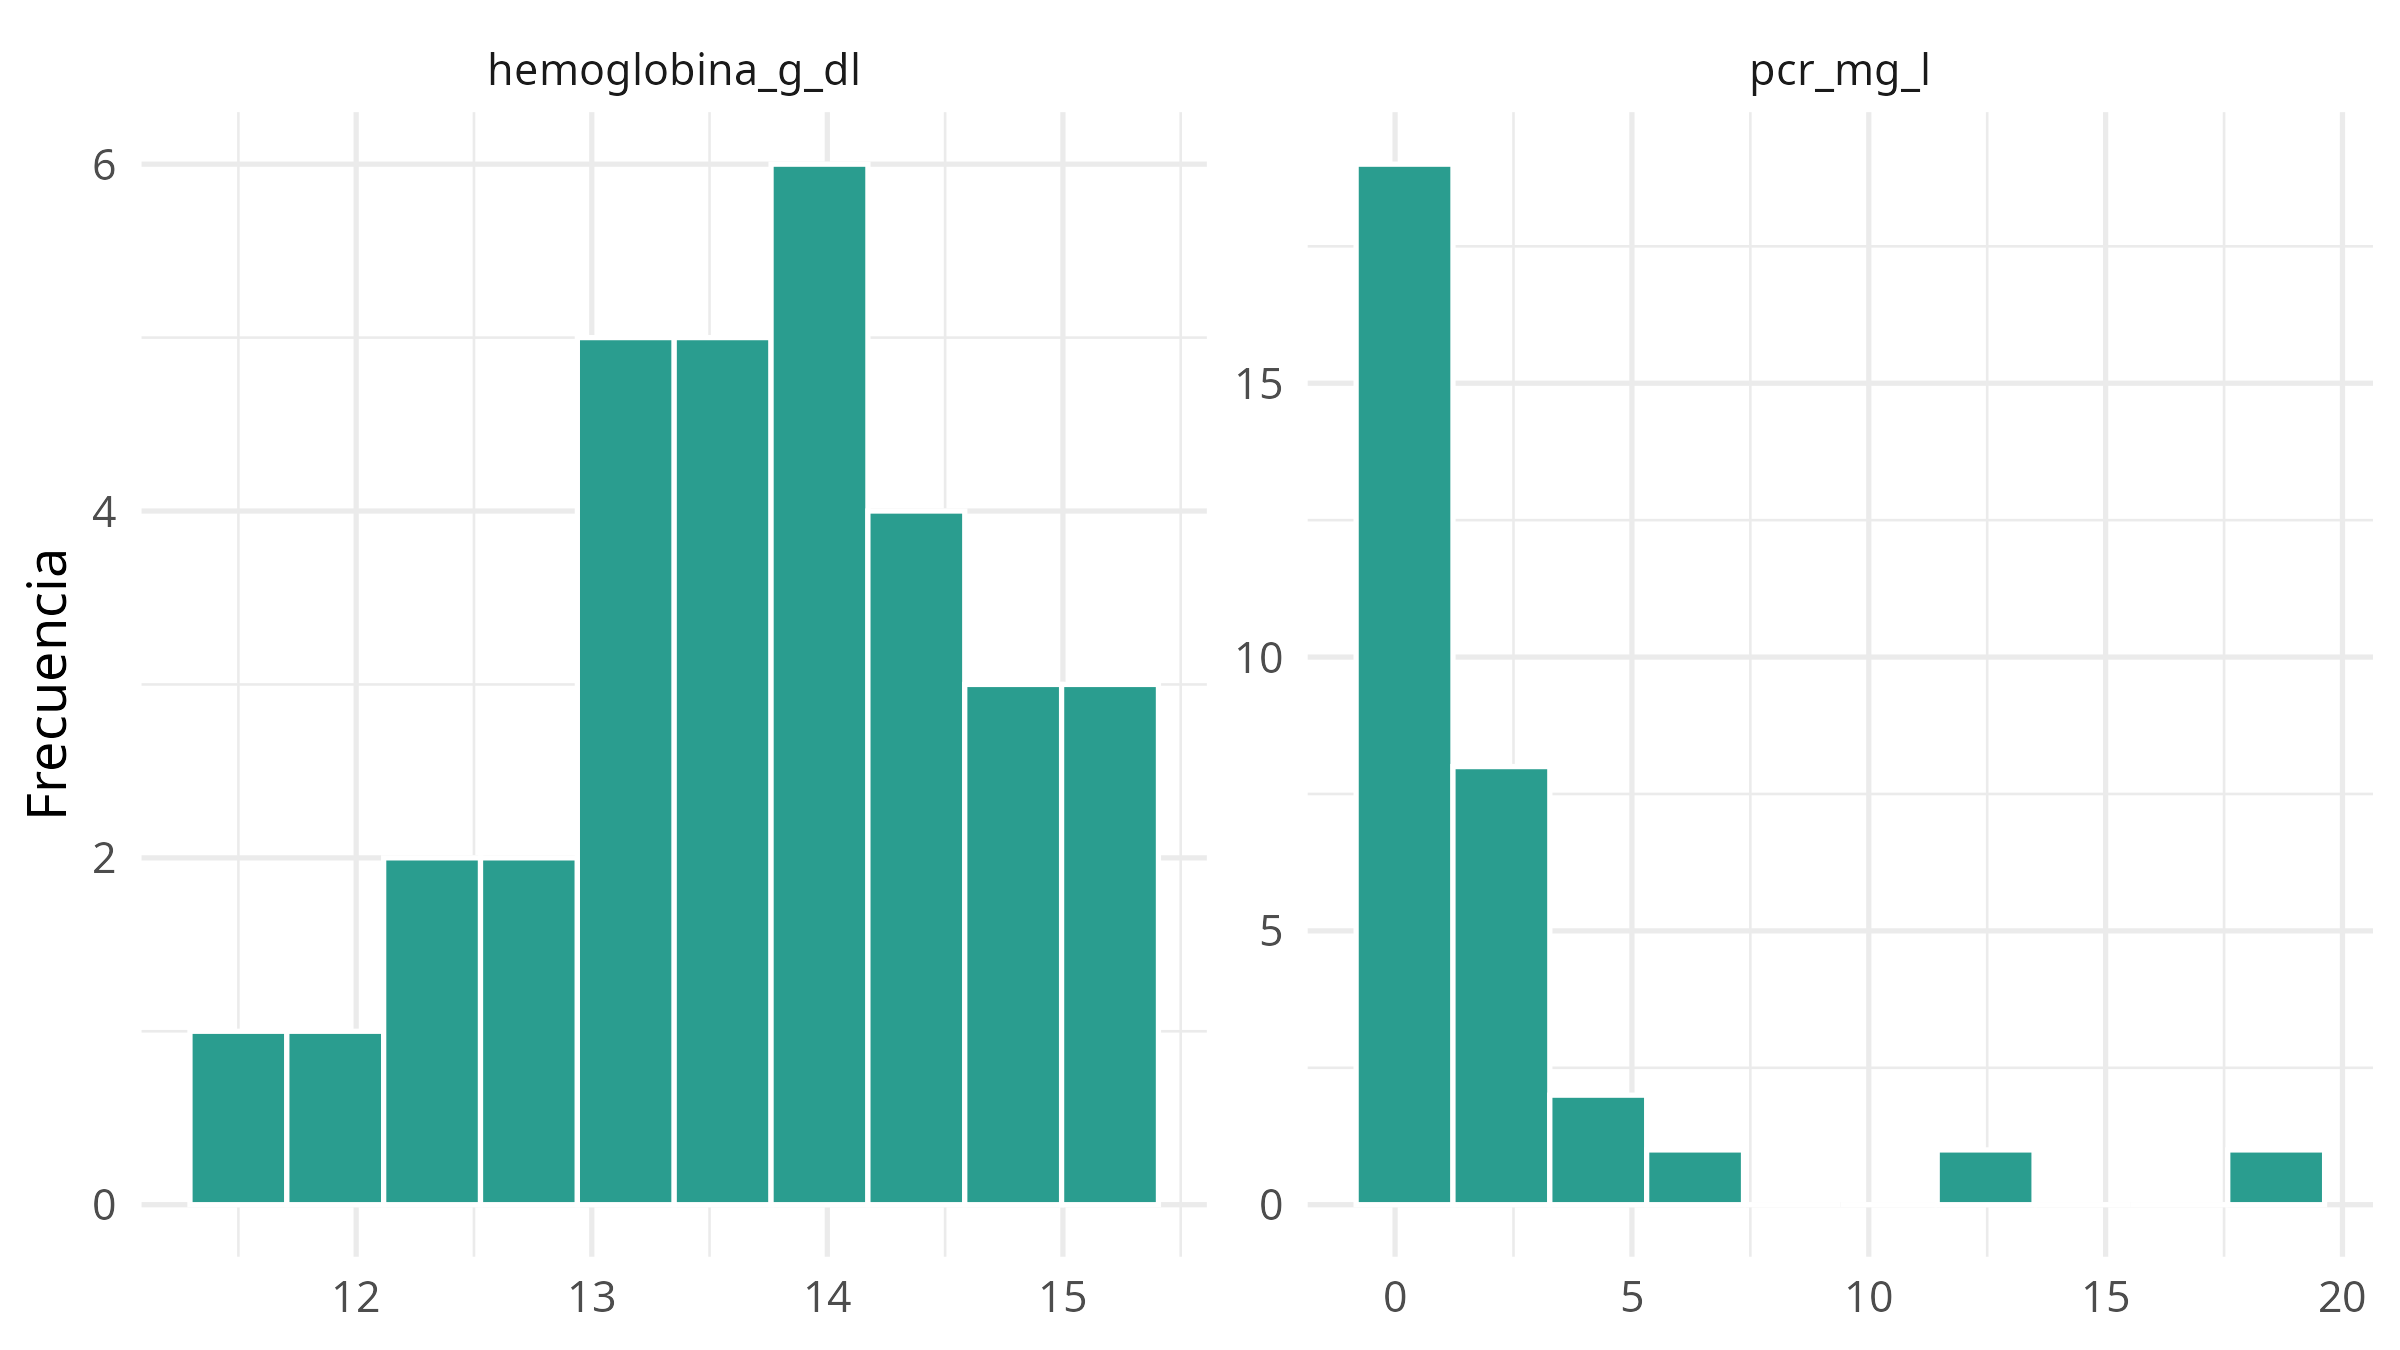
\includegraphics[width=\linewidth]{01_histogramas.png}
\end{columns}
\end{frame}

% 11
\begin{frame}[fragile]{Gráficos Q-Q}
\begin{columns}[T,onlytextwidth]
  \column{0.42\textwidth}
\begin{lstlisting}[basicstyle=\ttfamily\footnotesize]
ggplot(datos_largos,
       aes(sample = valor)) +
  stat_qq() +
  stat_qq_line() +
  facet_wrap(~ variable,
             scales = "free")
\end{lstlisting}
  \small Los puntos cercanos a la línea apoyan normalidad.
  \column{0.56\textwidth}
  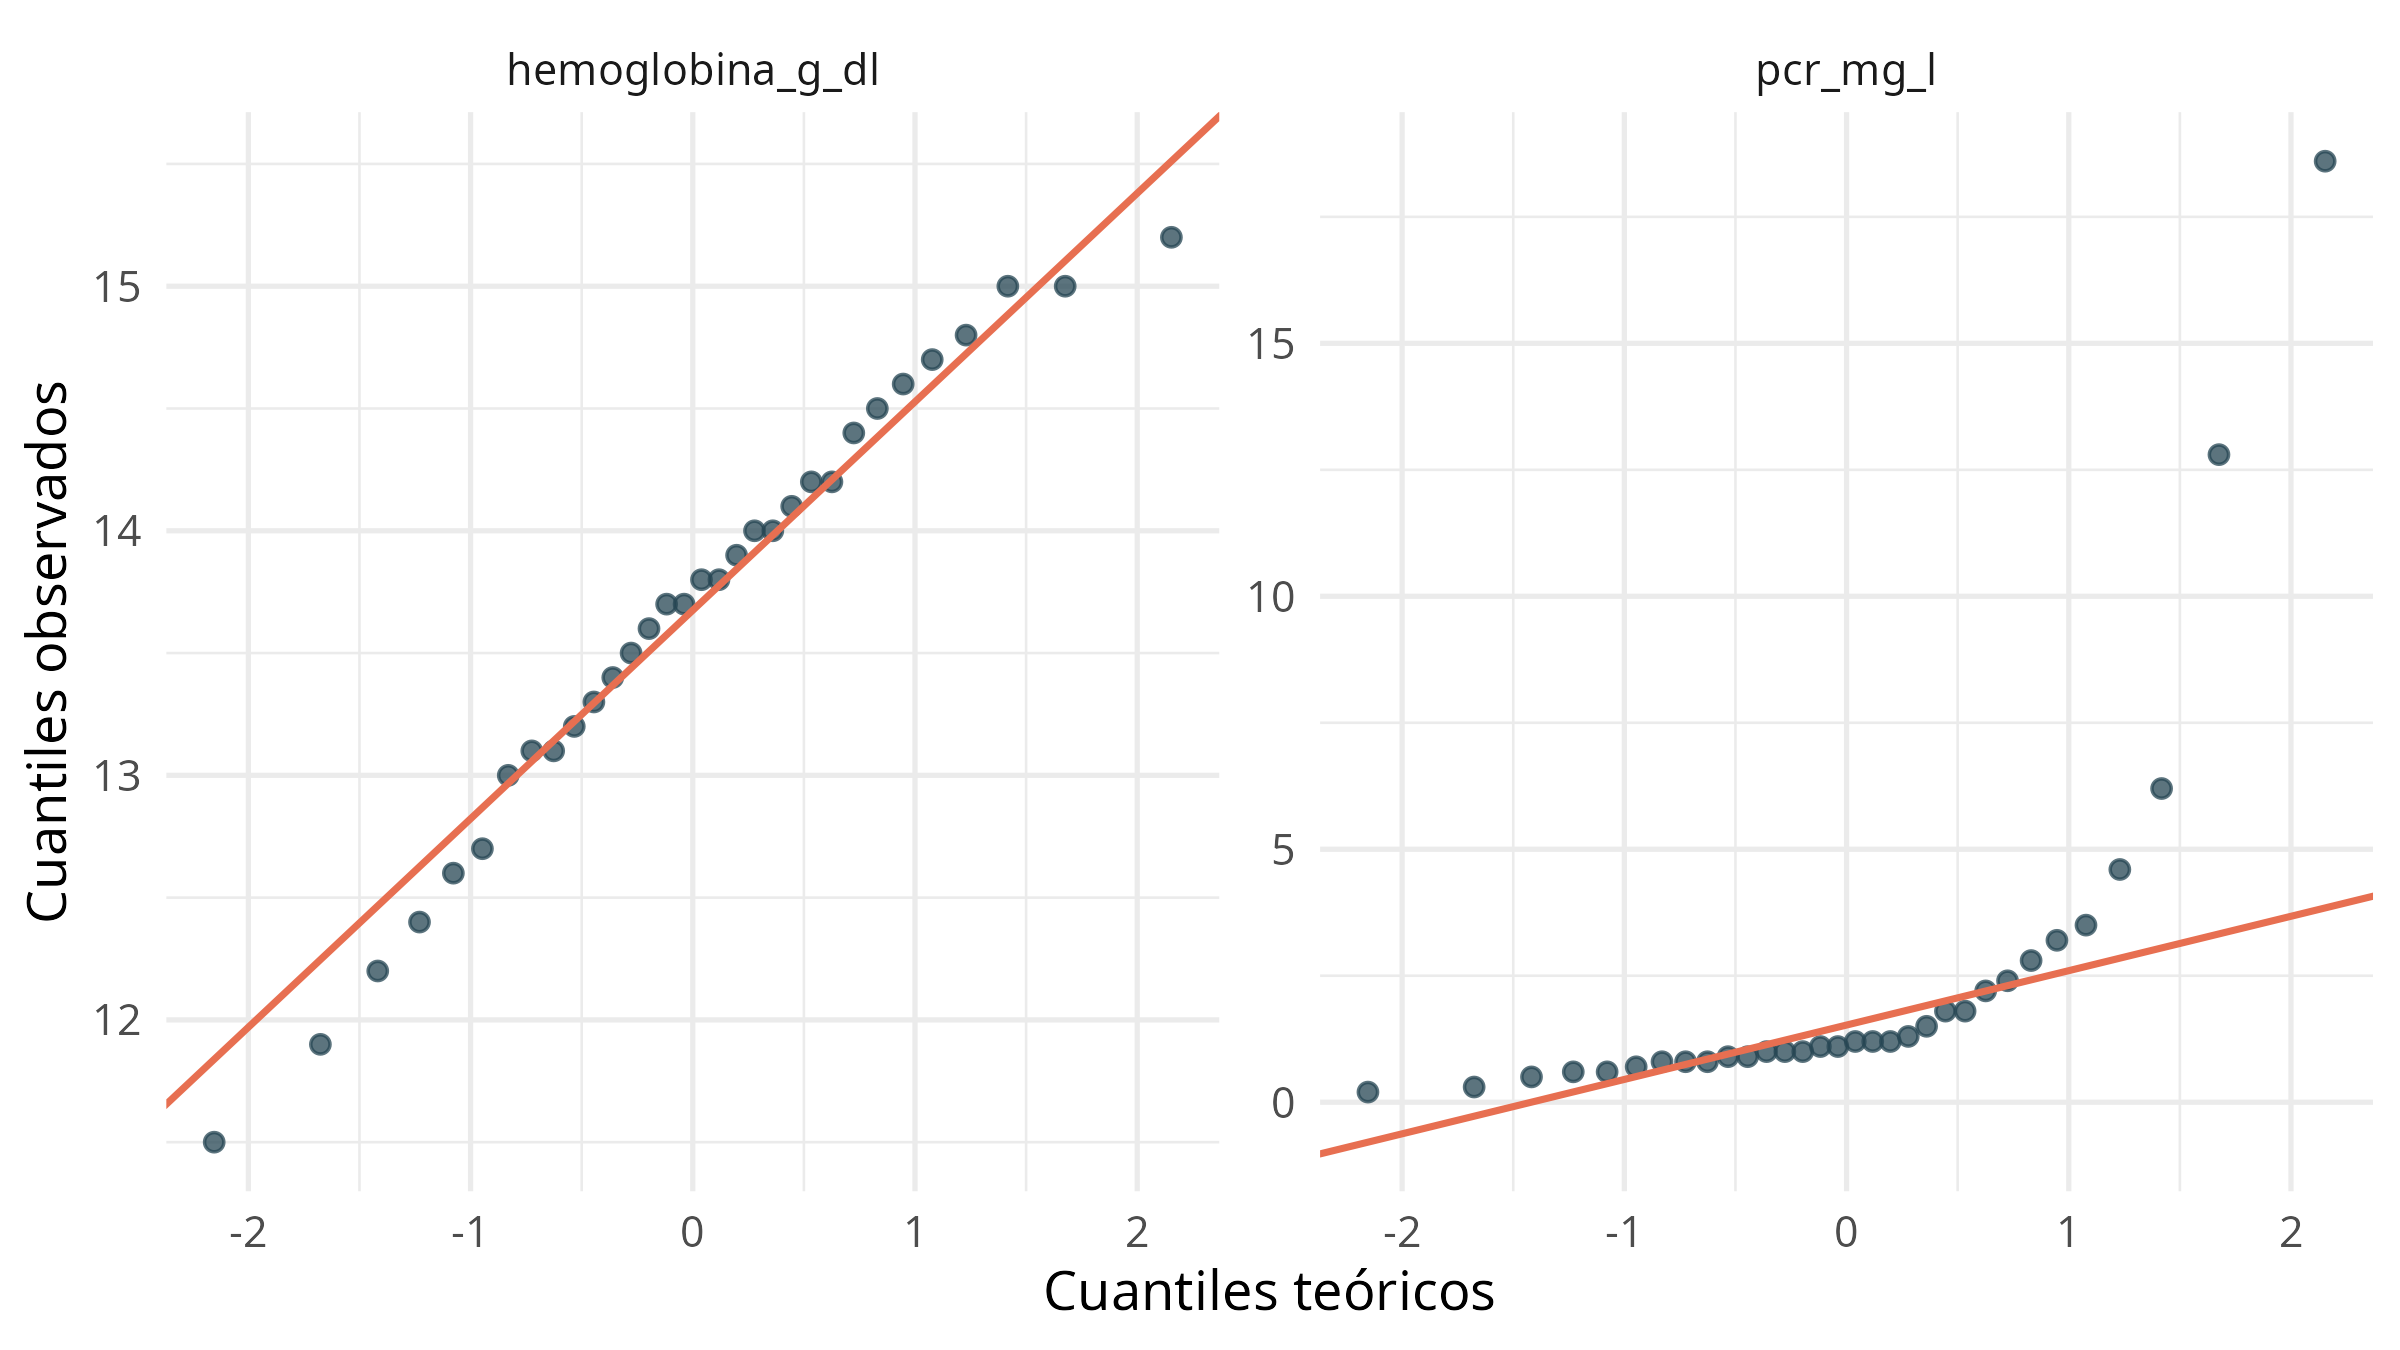
\includegraphics[width=\linewidth]{02_graficos_qq.png}
\end{columns}
\end{frame}

% 12
\begin{frame}{Shapiro-Wilk como apoyo a la decisión}
\large
\textbf{H$_0$:} los datos son compatibles con una distribución normal.

\vspace{0.6cm}
\begin{tabular}{lll}
\toprule
Resultado & Decisión práctica & Resumen sugerido\\
\midrule
$p \geq 0.05$ & No rechazamos H$_0$ & Media ± DE\\
$p < 0.05$ & Rechazamos H$_0$ & Mediana (Q1--Q3)\\
\bottomrule
\end{tabular}

\vspace{0.6cm}
\small El valor $p$ se interpreta junto con el histograma, el gráfico Q-Q y el contexto biológico.
\end{frame}

% 13
\begin{frame}[fragile]{Prueba de normalidad en R}
\begin{lstlisting}[basicstyle=\ttfamily\footnotesize]
normalidad <- datos_largos |>
  group_by(variable) |>
  summarise(
    W = unname(shapiro.test(valor)$statistic),
    p = shapiro.test(valor)$p.value
  )
\end{lstlisting}

\vspace{0.25cm}
\begin{tabular}{lrrl}
\toprule
Variable & W & p & Lectura\\
\midrule
Hemoglobina & 0.977 & 0.713 & Compatible con normalidad\\
PCR & 0.531 & $<0.001$ & Distribución asimétrica\\
\bottomrule
\end{tabular}
\end{frame}

% 14
\begin{frame}{Dos formas de resumir una variable}
\begin{columns}[T,onlytextwidth]
  \column{0.47\textwidth}
  {\color{verde}\Large\textbf{Paramétrica}}\\[0.3cm]
  Media: centro aritmético\\
  DE: dispersión alrededor de la media\\[0.35cm]
  \textbf{Reporte:} media ± DE
  \column{0.47\textwidth}
  {\color{naranja}\Large\textbf{No paramétrica}}\\[0.3cm]
  Mediana: observación central\\
  RIQ: intervalo de Q1 a Q3\\[0.35cm]
  \textbf{Reporte:} mediana (Q1--Q3)
\end{columns}

\vspace{0.8cm}
\centering
\large Calculamos ambas para aprender. Reportamos la que corresponde a la distribución.
\end{frame}

% 15
\begin{frame}[fragile]{Cálculo de los descriptivos}
\begin{lstlisting}[basicstyle=\ttfamily\footnotesize]
descriptivos <- datos_largos |>
  group_by(variable, grupo) |>
  summarise(
    n = n(),
    media = mean(valor), DE = sd(valor),
    mediana = median(valor),
    Q1 = quantile(valor, 0.25),
    Q3 = quantile(valor, 0.75)
  )
\end{lstlisting}
\end{frame}

% 16
\begin{frame}[plain]
\centering
\vfill
{\color{naranja}\fontsize{19}{22}\selectfont SESIÓN 2}\par
\vspace{0.25cm}
{\color{azul}\fontsize{30}{34}\selectfont De los resultados al reporte}\par
\vfill
\end{frame}

% 17
\begin{frame}{Anatomía de una tabla académica}
\large
\begin{itemize}
  \item Número y título breve encima de la tabla.
  \item Unidades dentro de los encabezados.
  \item Tamaño muestral visible.
  \item Pocas líneas horizontales y ningún adorno innecesario.
  \item Abreviaturas explicadas en una nota.
\end{itemize}

\vspace{0.5cm}
\small Vancouver regula principalmente las referencias. La revista define los detalles de sus tablas.
\end{frame}

% 18
\begin{frame}[fragile]{Construcción de la tabla con gt}
\begin{lstlisting}[basicstyle=\ttfamily\footnotesize]
tabla_academica <- tabla_reporte |>
  gt(groupname_col = "medida") |>
  cols_label(
    grupo = "Grupo clínico",
    resultado = "Resumen",
    p_shapiro = "p de Shapiro-Wilk"
  ) |>
  tab_header(title = "Tabla 1. Estadística descriptiva")
\end{lstlisting}

\small El script exporta versiones HTML, CSV y LaTeX.
\end{frame}

% 19
\begin{frame}{Tabla 1. Estadística descriptiva de los biomarcadores}
\scriptsize
\begin{tabular}{llrlll}
\toprule
Medida & Grupo & n & Resumen & $p$ & Reporte\\
\midrule
Hemoglobina & Control & 10 & 14.00 ± 0.80 & 0.713 & Media ± DE\\
Hemoglobina & Activa & 11 & 13.40 ± 1.02 & 0.713 & Media ± DE\\
Hemoglobina & Estable & 11 & 13.61 ± 0.93 & 0.713 & Media ± DE\\
\midrule
PCR & Control & 10 & 0.8 (0.5--1.0) & $<0.001$ & Mediana (Q1--Q3)\\
PCR & Activa & 11 & 2.8 (1.5--5.4) & $<0.001$ & Mediana (Q1--Q3)\\
PCR & Estable & 11 & 1.2 (0.9--1.6) & $<0.001$ & Mediana (Q1--Q3)\\
\bottomrule
\end{tabular}

\vspace{0.35cm}
\footnotesize DE: desviación estándar. Q1--Q3: rango intercuartílico. Normalidad evaluada por variable.
\end{frame}

% 20
\begin{frame}[fragile]{Gráfico para una variable normal}
\begin{columns}[T,onlytextwidth]
  \column{0.48\textwidth}
\begin{lstlisting}[basicstyle=\ttfamily\scriptsize]
ggplot(datos_limpios,
       aes(grupo, hemoglobina_g_dl,
           color = grupo)) +
  geom_jitter(width = 0.12) +
  stat_summary(fun = mean,
               geom = "point") +
  stat_summary(fun.data = mean_sdl,
               geom = "errorbar")
\end{lstlisting}
  \small Mostramos datos individuales, media y DE.
  \column{0.50\textwidth}
  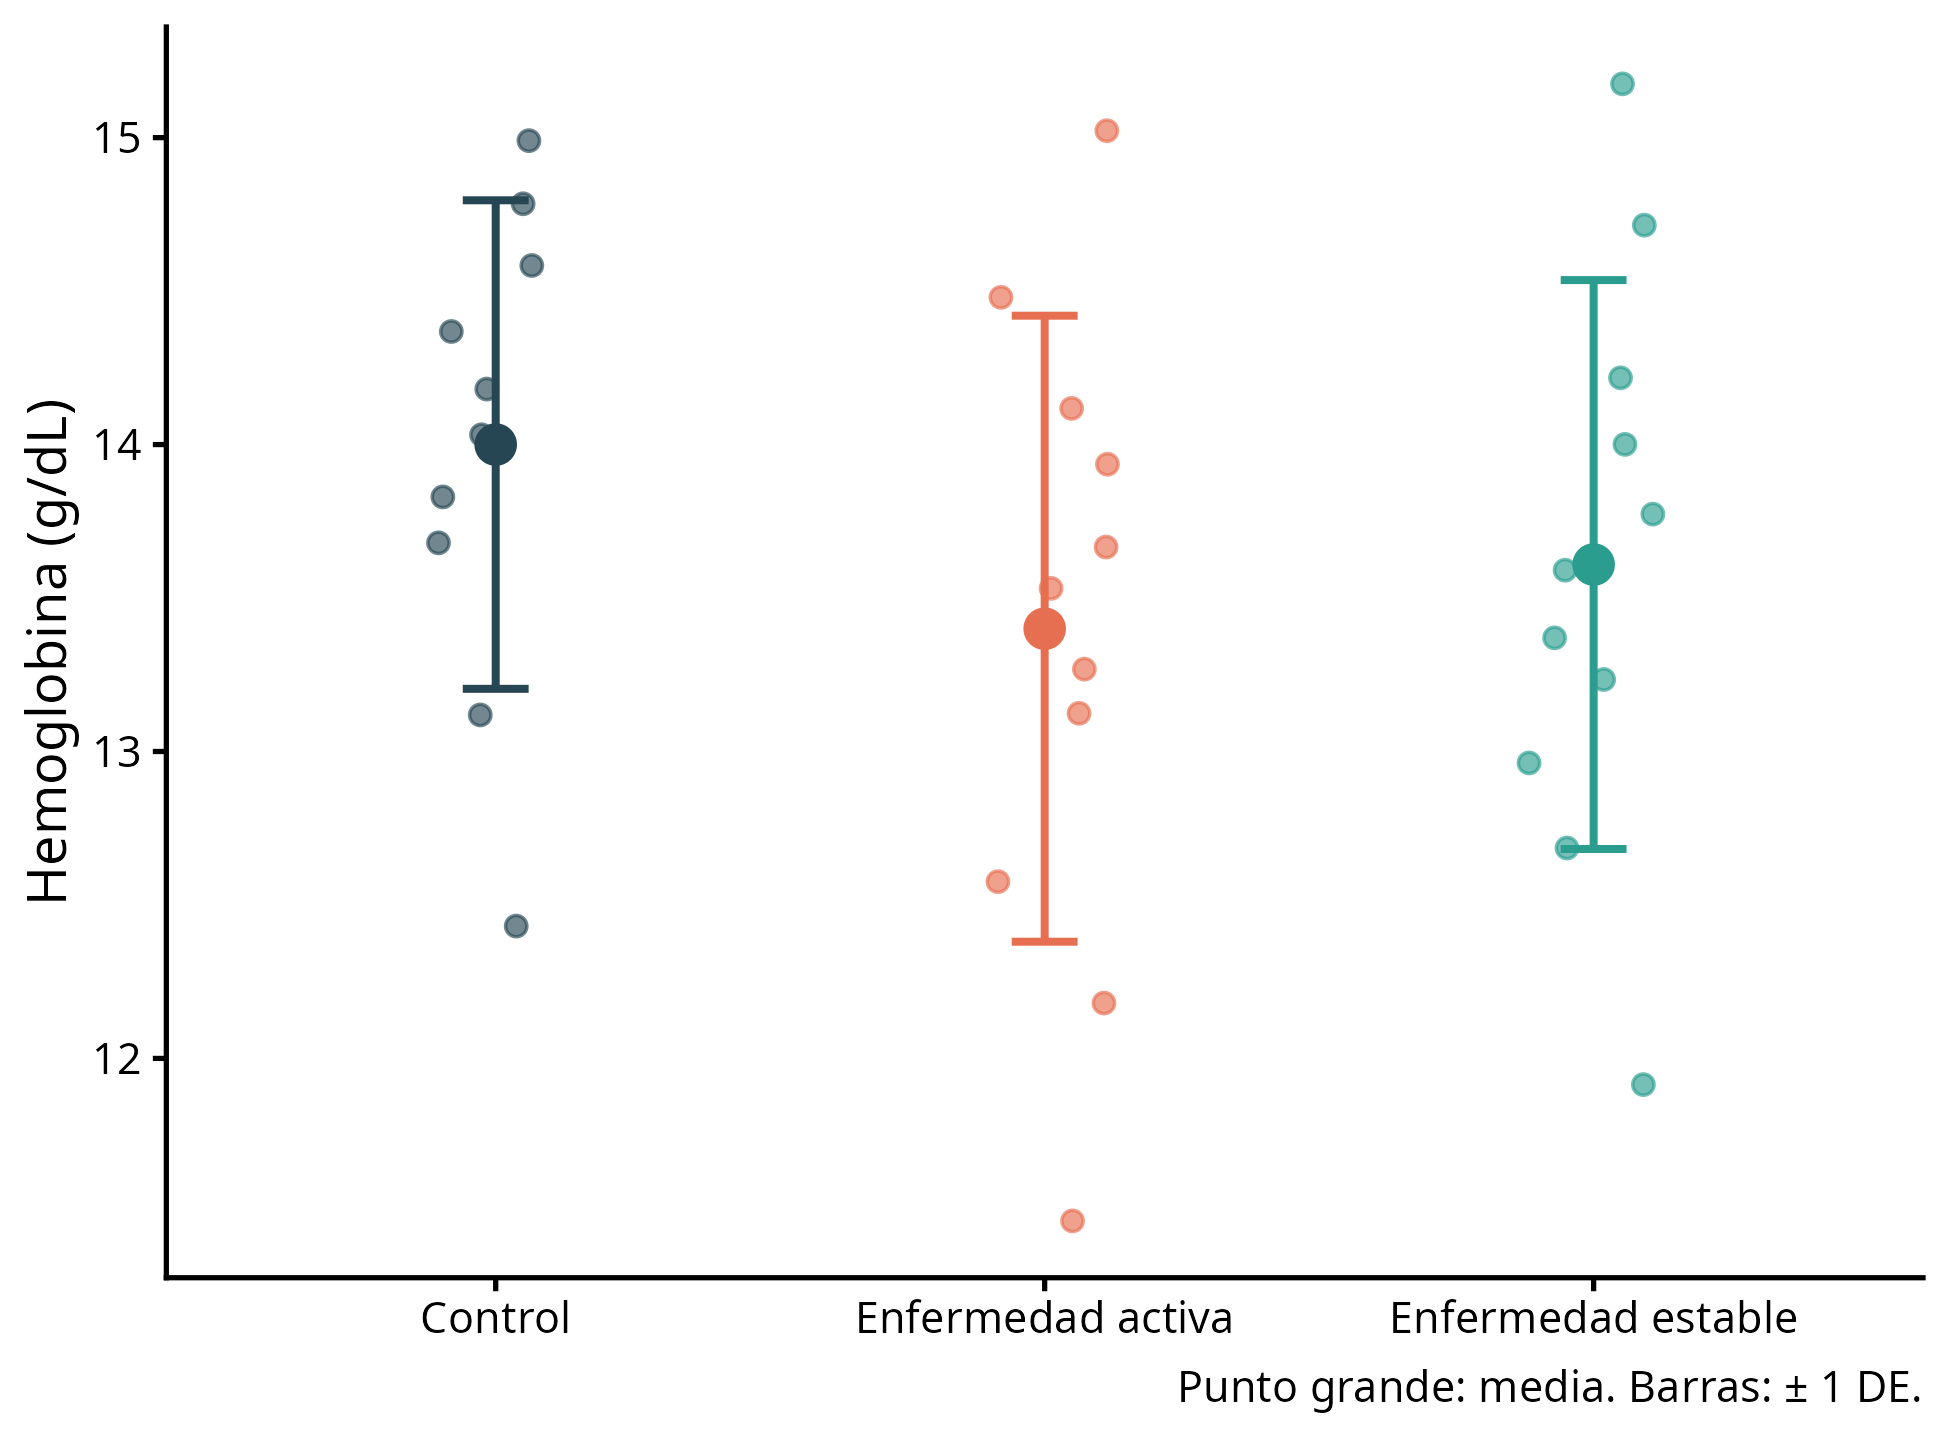
\includegraphics[width=\linewidth]{03_hemoglobina_media_DE.png}
\end{columns}
\end{frame}

% 21
\begin{frame}[fragile]{Gráfico para una variable asimétrica}
\begin{columns}[T,onlytextwidth]
  \column{0.48\textwidth}
\begin{lstlisting}[basicstyle=\ttfamily\scriptsize]
ggplot(datos_limpios,
       aes(grupo, pcr_mg_l,
           fill = grupo)) +
  geom_boxplot(
    outlier.shape = NA,
    alpha = 0.45
  ) +
  geom_jitter(width = 0.12)
\end{lstlisting}
  \small La caja muestra mediana y RIQ. Los puntos conservan la información original.
  \column{0.50\textwidth}
  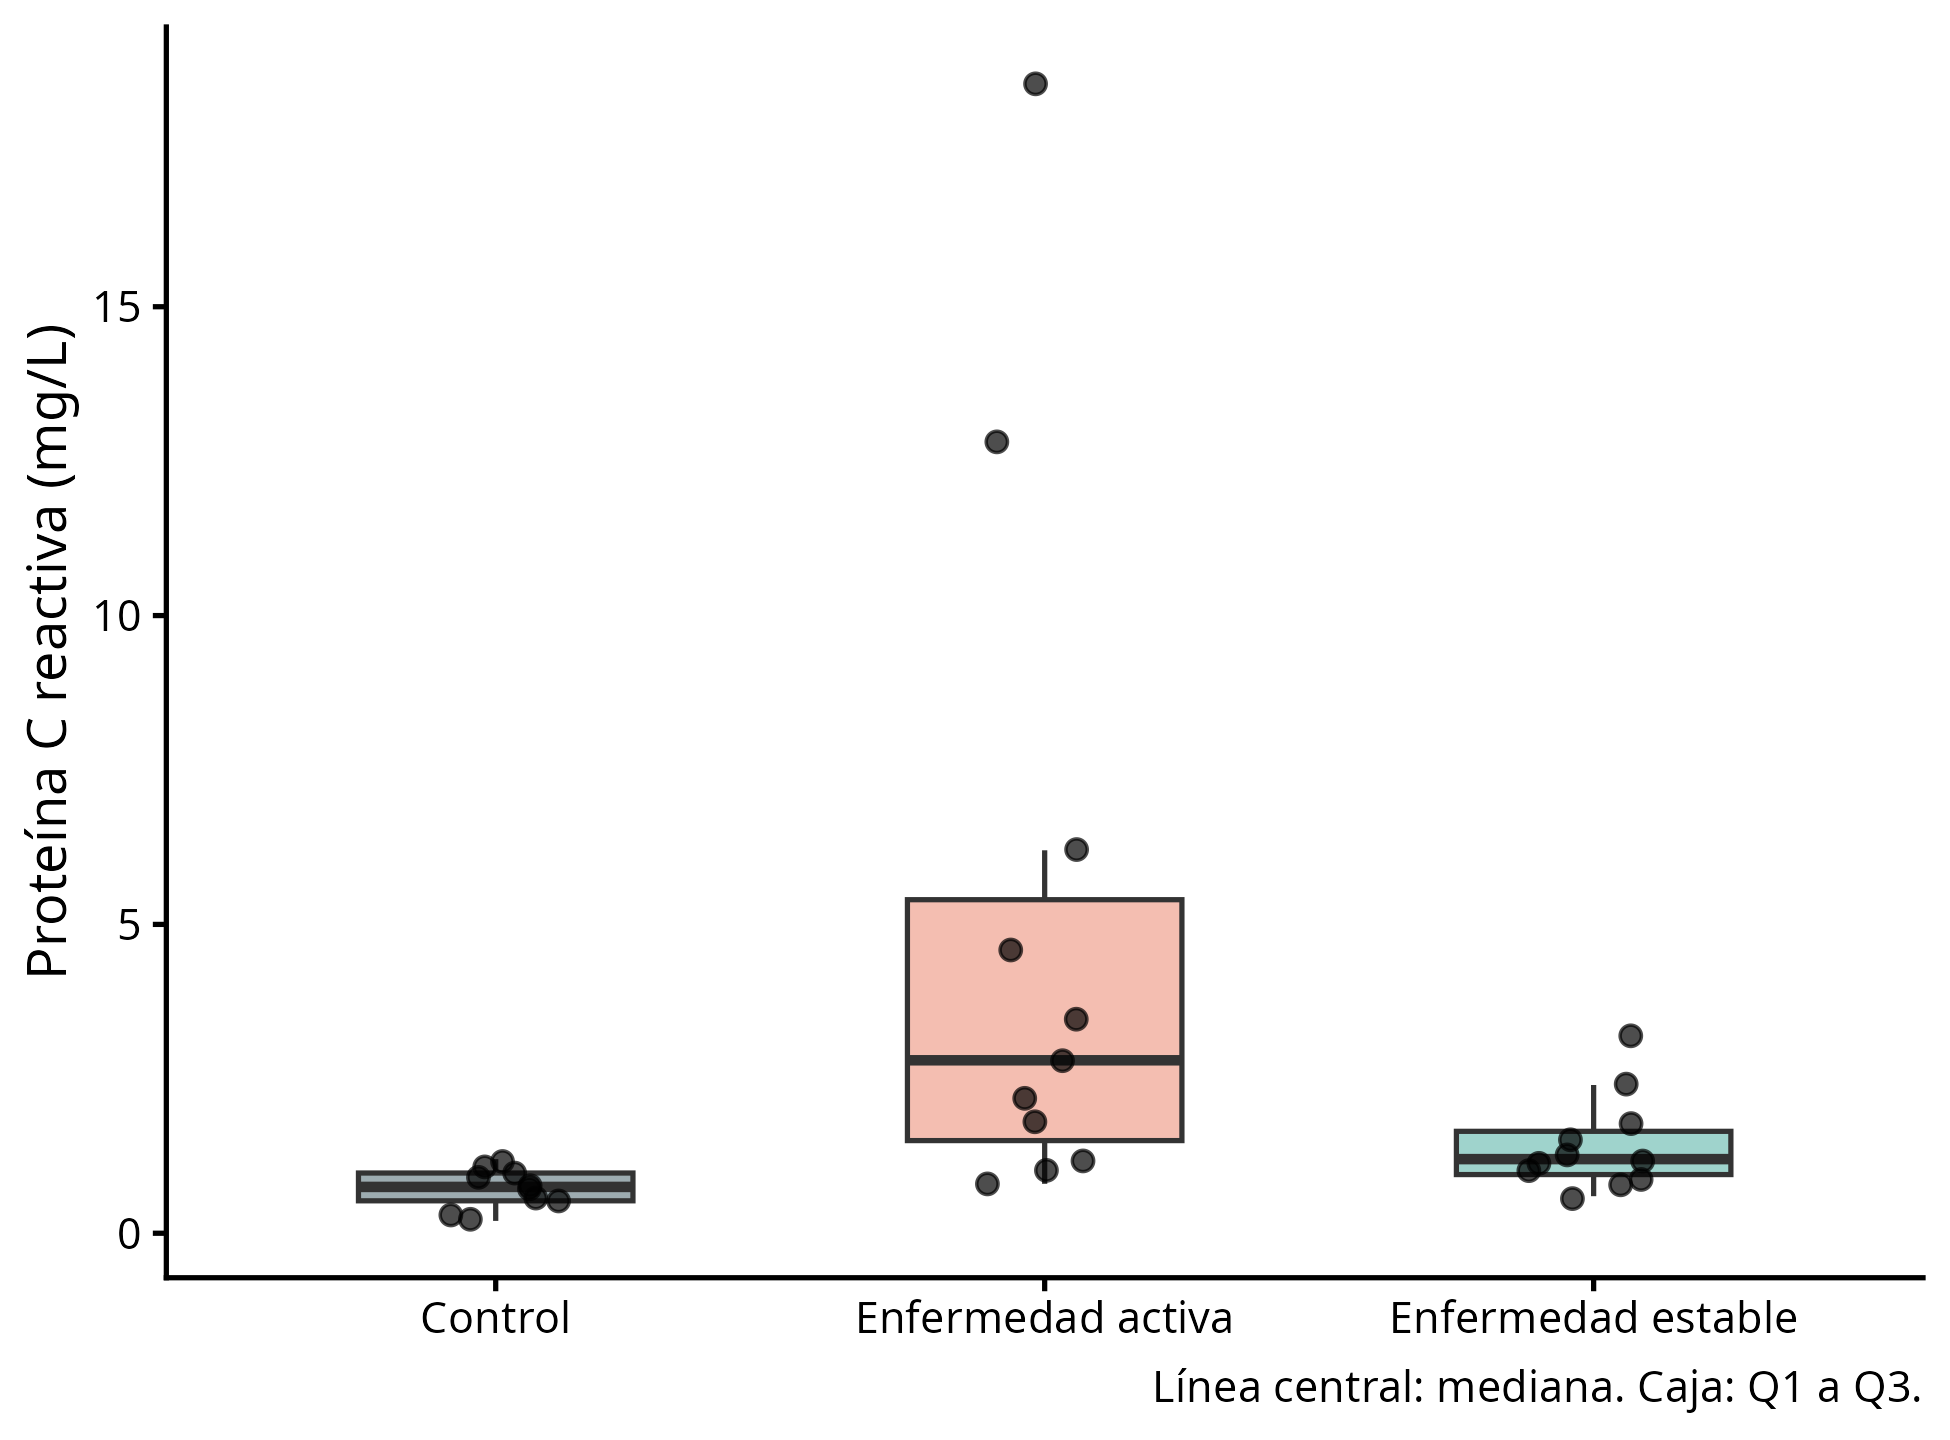
\includegraphics[width=\linewidth]{04_pcr_mediana_RIQ.png}
\end{columns}
\end{frame}

% 22
\begin{frame}{Redacción de los resultados}
\begin{block}{Variable compatible con normalidad}
La hemoglobina fue compatible con una distribución normal (Shapiro-Wilk, W = 0.977, p = 0.713), por lo que se resumió como media ± DE.
\end{block}

\begin{block}{Variable asimétrica}
La proteína C reactiva mostró una distribución asimétrica (Shapiro-Wilk, W = 0.531, p $< 0.001$), por lo que se resumió como mediana (Q1--Q3).
\end{block}

\small Estas frases describen los datos. Todavía no prueban diferencias entre grupos clínicos.
\end{frame}

% 23
\begin{frame}{Límites de esta primera aproximación}
\begin{itemize}
  \item Shapiro-Wilk no reemplaza la inspección visual.
  \item Una muestra pequeña puede ocultar desviaciones de normalidad.
  \item Una muestra grande puede detectar desviaciones poco importantes.
  \item Eliminar NA puede introducir sesgo si la ausencia no ocurre al azar.
  \item En análisis inferencial suele evaluarse la distribución de los residuos.
\end{itemize}

\vspace{0.4cm}
\large La decisión estadística también depende de la pregunta y del diseño experimental.
\end{frame}

% 24
\begin{frame}{Práctica de cierre}
\large
Cambie una parte del flujo y vuelva a ejecutarlo:

\vspace{0.35cm}
\begin{enumerate}
  \item Añada una variable biológica nueva al CSV.
  \item Prediga si su distribución será simétrica o asimétrica.
  \item Genere histograma, Q-Q y Shapiro-Wilk.
  \item Produzca el resumen y el gráfico correspondientes.
\end{enumerate}

\vspace{0.5cm}
\centering
\textcolor{verde}{\Large\textbf{La meta es reproducir el flujo y explicar cada decisión.}}
\end{frame}

% 25
\begin{frame}{Recursos para continuar}
\small
\begin{thebibliography}{9}
\bibitem{ghasemi}
Ghasemi A, Zahediasl S. Normality tests for statistical analysis: a guide for non-statisticians. Int J Endocrinol Metab. 2012;10(2):486--489.

\bibitem{wickham}
Wickham H. ggplot2: Elegant Graphics for Data Analysis. 2nd ed. Cham: Springer; 2016.

\bibitem{r}
R Core Team. R: A language and environment for statistical computing. Vienna: R Foundation for Statistical Computing.
\end{thebibliography}

\vfill
\centering
\textcolor{azul}{El script completo contiene comentarios, exportaciones y frases modelo.}
\end{frame}

\end{document}
